\documentclass{article}
\usepackage{graphicx} % Required for inserting images
% Used added packages
\usepackage[shortlabels]{enumitem}
\usepackage{blindtext}
\usepackage[export]{adjustbox}
\usepackage{wrapfig, siunitx, caption, subcaption, multirow, nicefrac}
\usepackage{color,soul}

\usepackage[english]{babel}

\usepackage{hyperref}
\usepackage{arsclassica} % Modifies the Classic Thesis package

\usepackage[T1]{fontenc} % Use 8-bit encoding that has 256 glyphs

\usepackage[utf8]{inputenc} % Required for including letters with accents

\usepackage{graphicx} % Required for including images
\graphicspath{{Figures/}} % Set the default folder for images

\usepackage{enumitem} % Required for manipulating the whitespace between and within lists

\usepackage{lipsum} % Used for inserting dummy 'Lorem ipsum' text into the template

% \usepackage{subfig} % Required for creating figures with multiple parts (subfigures)

\usepackage{amsmath,amssymb,amsthm} % For including math equations, theorems, symbols, etc

\usepackage{varioref} % More descriptive referencing

\usepackage{listings}

\usepackage{epstopdf}
\usepackage[numbers]{natbib}
\usepackage{float}
\usepackage{emptypage}


\usepackage{booktabs}
\usepackage[ruled,vlined,linesnumbered]{algorithm2e}
% Custom right-aligned quote environment
\newcommand{\rightquote}[2]{
  \begin{flushright}
    \parbox{0.6\textwidth}{\raggedleft
      #1\vspace{0.1ex}\\
      \rule{0.55\textwidth}{0.4pt}\\
      \textit{#2}
    }
  \end{flushright}
}

\usepackage{chngcntr}

%\usepackage{subcaption}
\usepackage{nomencl}
\makenomenclature

\definecolor{AUpantone}{rgb}{0.0, 0.2392156, 0.5111111}
\definecolor{AUpantoneDark}{rgb}{0.0, 0.1450980392156863, 0.27450980392156865}
\definecolor{AUpantoneCyan}{rgb}{0.21568627, 0.6274509, 0.79607843}
\definecolor{AUpantoneTurkis}{rgb}{0.0, 0.6705882353, 0.6431372549}


\newenvironment{dedication}
  {\clearpage           % we want a new page
   \thispagestyle{empty}% no header and footer
   \vspace*{\stretch{1}}% some space at the top 
   \itshape             % the text is in italics
   \raggedleft          % flush to the right margin
  }
  {\par % end the paragraph
   \vspace{\stretch{3}} % space at the bottom is three times that at the top
   \clearpage           % finish off the page
  }


\titleformat{\chapter}[display]%
  {\relax}{\vspace*{-3\baselineskip}\makebox[\linewidth][r]{\color{AUpantoneDark}\chapterNumber\thechapter}}{0pt}%
  {\raggedright\spacedallcaps}[\normalsize\vspace*{.8\baselineskip}\titlerule]%

  % {\raggedright\spacedallcaps}[\normalsize\vspace*{.8\baselineskip}]%
  
%---------------------------------------------------------------------------------------
%      CODE
%---------------------------------------------------------------------------------------
\lstdefinestyle{mystyle}{
    basicstyle=\footnotesize,
    breakatwhitespace=true,         
    breaklines=true,                 
    captionpos=b,                    
    keepspaces=true,                 
    numbers=left,                    
    numbersep=5pt,                  
    showspaces=false,                
    showstringspaces=false,
    showtabs=false,                  
    tabsize=2
}
\lstset{style=mystyle}

%----------------------------------------------------------------------------------------
%	THEOREM STYLES
%---------------------------------------------------------------------------------------

\theoremstyle{definition} % Define theorem styles here based on the definition style (used for definitions and examples)
\newtheorem{Def}{Definition}

\theoremstyle{plain} % Define theorem styles here based on the plain style (used for theorems, lemmas, propositions)
\newtheorem{Th}{Theorem}
\newtheorem{Cor}[Th]{Corollary}
\newtheorem{Lemma}[Th]{Lemma}
\newtheorem{Ex}[Th]{Example}
\newtheorem{Oss}[Th]{Remark}

\theoremstyle{remark} % Define theorem styles here based on the remark style (used for remarks and notes)

%----------------------------------------------------------------------------------------
%	HYPERLINKS
%---------------------------------------------------------------------------------------

\hypersetup{
%draft, % Uncomment to remove all links (useful for printing in black and white)
colorlinks=true, breaklinks=true, bookmarksnumbered,
urlcolor=AUpantone, linkcolor=AUpantone, citecolor=AUpantone, % Link colors
pdftitle={simone_manti_phd_thesis}, % PDF title
pdfauthor={\textcopyright}, % PDF Author
pdfsubject={A Discrete Geometric Approach to Data-Driven
Model Discovery}, % PDF Subject
pdfkeywords={}, % PDF Keywords
pdfcreator={pdfLaTeX}, % PDF Creator
pdfproducer={LaTeX with hyperref and ClassicThesis} % PDF producer
}
% Other functions
\newcommand{\vect}[1]{\mathbf{#1}}%In order to show vectors in bold

\usepackage{appendix}
\usepackage{titlesec}



% C++ typeset in appendix
\usepackage{listings}
\usepackage{xcolor} % for setting colors
\usepackage{minted}

% Use a dark VS Code-style theme
\usemintedstyle{monokai}


% Optional: set dark background for code blocks
\definecolor{bg}{rgb}{0.17,0.17,0.17} % VS Code dark background
\definecolor{lightgray}{rgb}{0.95,0.95,0.95}


% set the default code style
\lstset{
    % frame=tb, % draw a frame at the top and bottom of the code block
    tabsize=4, % tab space width
    showstringspaces=false, % don't mark spaces in strings
    numbers=left, % display line numbers on the left
    commentstyle=\color{green}, % comment color
    keywordstyle=\color{blue}, % keyword color
    stringstyle=\color{red} % string color
}

\usepackage[
top    = 2.00cm,
bottom = 2.00cm,
left   = 2.00cm,
right  = 2.00cm]{geometry}

\usepackage{bbm}
\usepackage{amscd}
\usepackage{pdfpages}
\usepackage{longtable}
\usepackage{tabularx}
\usepackage{tikz}
\usetikzlibrary{positioning}


\newcommand{\defeq}{\vcentcolon=}
\newcommand{\im}{\operatorname{im}}
\newcommand{\Hom}{{\rm{Hom}}}
\newcommand{\diam}{{\rm{diam}}}
\newcommand{\dom}{\text{dom}}
\newcommand{\ovl}{\overline}
\newcommand{\rr}{\mathbb{R}}
\newcommand{\EE}{\mathcal{E}}
\newcommand{\VV}{\mathcal{V}}
\newcommand{\mystar}{{\fontfamily{lmr}\selectfont$\star$}}
\newcommand{\llangle}{\langle \langle}
\newcommand{\rrangle}{\rangle \rangle}

%bold commands
\newcommand{\xx}{\mathbf{x}}
\newcommand{\Xx}{\mathbf{X}}
\newcommand{\Tt}{\mathbf{T}}
\newcommand{\yy}{\mathbf{y}}
\newcommand{\ee}{\mathbf{e}}
\newcommand{\cc}{\mathbf{c}}
\newcommand{\uu}{\mathbf{u}}
\newcommand{\vv}{\mathbf{v}}
\newcommand{\ww}{\mathbf{w}}
\newcommand{\om}{\boldsymbol{\omega}}
\newcommand{\al}{\boldsymbol{\alpha}}
\newcommand{\be}{\boldsymbol{\beta}}
\newcommand{\ta}{\boldsymbol{\tau}}


%calcommand

\newcommand{\mc}{\mathcal}


% Command to create a title page for each eer
\newcommand{\papertitlepage}[5]{%
  \cleardoublepage
  \thispagestyle{empty}
  % Save the current geometry
  \newgeometry{
    top=2.5cm,
    bottom=2.5cm,
    left=3cm,
    right=3cm
  }
  
  % Title page content here
  \begin{center}
    \Large\textbf{Paper #1}\\[1cm]
    \LARGE\textbf{#2}\\[1cm]
    \large{#3}\\[1cm]
    \normalsize{#4}\\[0.5cm]
    \small{#5}
  \end{center}
  
  % Restore the original geometry
  \restoregeometry
}

\DeclareMathOperator*{\argmax}{arg\,max}
\DeclareMathOperator*{\argmin}{arg\,min}

\title{Discrete Exterior Calculus}
\author{Simone Manti}
\date{January 2026}

\begin{document}

\maketitle

Exterior Calculus (EC) \cite{abraham2012manifolds}, also known as the calculus of differential forms, is a powerful mathematical framework for formulating and analyzing problems involving geometry and topology. Developed to generalize classical vector calculus, EC provides a coordinate-free approach particularly suited for manifold settings.

Central in EC is the concept of \textit{differential form}. Basically, a differential $k$-form is an object that can be integrated over $k$-dimensional manifolds. The primary operations in EC include:
\begin{itemize}
\item The \textbf{exterior derivative} $\mathrm{d}$: a generalization of gradient, curl, and divergence.
\item The \textbf{wedge product} $\wedge$: an associative, bilinear, and antisymmetric product of forms.
\item The \textbf{Hodge star} $\star$: maps $k$-forms to $(n-k)$-forms on an $n$-dimensional oriented Riemannian manifold.
\end{itemize}
EC provides a general and unified approach, which is particularly useful in fields such as differential geometry, topology, and theoretical physics. Table~\ref{tab: vc_vs_ec} shows a comparison between vector and exterior calculus.

While EC provides a powerful and elegant continuous framework, a discrete counterpart is needed for practical applications (\textsl{e.g.}, in computational physics).
Discrete Exterior Calculus (DEC) \cite{hirani2003discrete, desbrun2005discrete} is exactly the discrete version of EC. It operates on simplicial complexes (which play the role of the manifolds for EC) and maintains the geometric and topological structure of the continuous counterpart. 
Most importantly, DEC is inherently a discrete framework that bypasses the need for a differential formulation of physical theories. As a result, local conservation laws are naturally and strongly enforced, without requiring the discretization of differential operators \cite{tonti2013mathematical}.
In \cite{griebel2017upwind} the authors show that DEC can be specialized into other well-known numerical methods, such as Finite Volume Method and Finite Differences. Table~\ref{tab: fem_vs_dec} shows a comparison with DEC and the Finite Element Method (FEM), another popular choice for the discretization of Partial Differential Equations (PDE).

\begin{table}[ht!]
\centering
\begin{tabularx}{\textwidth}{@{}lXX@{}}
\toprule
\textbf{Feature} & \textbf{Vector Calculus} & \textbf{Exterior Calculus} \\ 
\midrule

Differentiation & $\nabla$, curl, div & Exterior derivative $\mathrm{d}$ \\
Integration domain &  $ \Omega \subset \mathbb{R}^n$ & $n$-manifolds\\
Variables & Vector fields & Differential forms \\
Product & Dot/cross products & Wedge product $\wedge$ \\
Stokes' theorem & Several variants & $\int_{\partial \Omega} \omega = \int_{\Omega} \mathrm{d}\omega$ \\
Operator identity & $\nabla \cdot (\nabla \times \mathbf{F}) = 0$ & $\mathrm{d}^2 = 0$ \\
%Coordinate dependence & Yes & No (coordinate-free) \\
Hodge star & Not used explicitly & Maps between dual degrees \\
Duality & Vector/tensor duality & $\star$ duality of forms \\

\bottomrule
\end{tabularx}
\caption{Overview of the key differences between vector and exterior calculus.}
\label{tab: vc_vs_ec}
\end{table}

This chapter is organized as follows. Section~\ref{sec: dec} presents the core concepts of DEC. Section~\ref{sec: dec_examples} collects some examples of application of DEC for different scenarios. Finally, Section~\ref{sec: dctkit} gives a gentle and concise introduction to the discrete calculus library \texttt{dctkit}, which provides a \texttt{python} implementation of the concepts described in this chapter.

Let us fix some notations used in the following sections: 
\begin{itemize}
    \item $\mathcal{E}^n$ is an $n$-dimensional euclidean space.
    \item $\mathcal{V}$ is the $n$-dimensional translation space of $\mathcal{E}^n$ with base $\{\ee_1, \dots, \ee_n\}$.
    \item $\llangle \cdot , \cdot \rrangle: \VV \times \VV \rightarrow \rr$ is an inner product, \textit{i.e.} a symmetric bilinear positive definite function.
\end{itemize}

\section{DEC Fundamentals}
\label{sec: dec}
\begin{table}[t!]
\centering
\begin{tabularx}{\textwidth}{@{}lXX@{}}
\toprule
\textbf{Feature} & \textbf{FEM} & \textbf{DEC} \\
\midrule
Mathematical foundation & Variational principles & Exterior calculus \\
Variables & Scalar/vector fields in $H^1$ & Cochains \\
Mesh structure & Triangular/quadrilateral & Simplicial complex\\
Differentiation & Weak derivatives & Coboundary \\
Metric dependency & In shape functions and integrals & In the Hodge star \\
Topological invariants & Not explicitly preserved & Naturally preserved \\
Local conservation laws & Enforced in weak form & Strongly enforced \\
\bottomrule
\end{tabularx}
\caption{Overview of the key differences between the Finite Element Method (FEM) and Discrete Exterior Calculus (DEC).}
\label{tab: fem_vs_dec}
\end{table}
In this section we provide a gentle introduction about the fundamentals of Discrete Exterior Calculus (DEC). For further details on DEC, the reader is referred to \cite{hirani2003discrete, grinspun2006discrete, desbrun2005discrete, crane2018discrete, grady2010discrete}.

\subsection{Discrete Domains}
\begin{Def}
        A \textbf{$p$-cell} $\sigma^p$ is defined as a set of points which is homeomorphic to a closed unit $p$-ball $B_p := \{x \in \rr^p | ||x|| \leq 1\}$. The boundary of the $p$-cell $\partial \sigma^p$ is the portion of the cell which is mapped through the homeomorphism to $\partial B_p$.
        When a $p$-cell consists of exactly $p+1$ vertices it is called \textbf{$p$-simplex}.
\end{Def}

We can think of a cell complex as the discrete counterpart of a manifold, in the sense that, within discrete calculus, it plays a role analogous to that of a manifold in classical exterior calculus. 
In fact, the following definition corresponds exactly to the concept of a discrete manifold in \cite{grinspun2006discrete} (see p.~43, Section~3.1.5). 
In \cite{hirani2003discrete}, such structures are referred to as \textsl{manifold-like cell complexes}. 

\begin{Def}
    A collection of cells defines a \textbf{cell complex} if it satisfies the following rules:
    \begin{itemize}
    \setlength\itemsep{0.01em}
        \item The boundary of each $p$-cell (for $p > 0$) comprises the union of lower-order $p$-cells.
        \item The intersection of any two cells is either empty or a boundary element of both cells.
    \end{itemize}
\end{Def}

A \textbf{simplicial complex} is a cell complex in which every $p$-cell is a $p$-simplex. In Figure~\ref{fig: sim_comp_example} we report an example of a 2-simplicial complex alongside an example of a non-simplicial complex. Notice that the latter is not a simplicial complex because the intersection of two $1$-cells is not a boundary element of both cells.

\begin{figure}[t!]
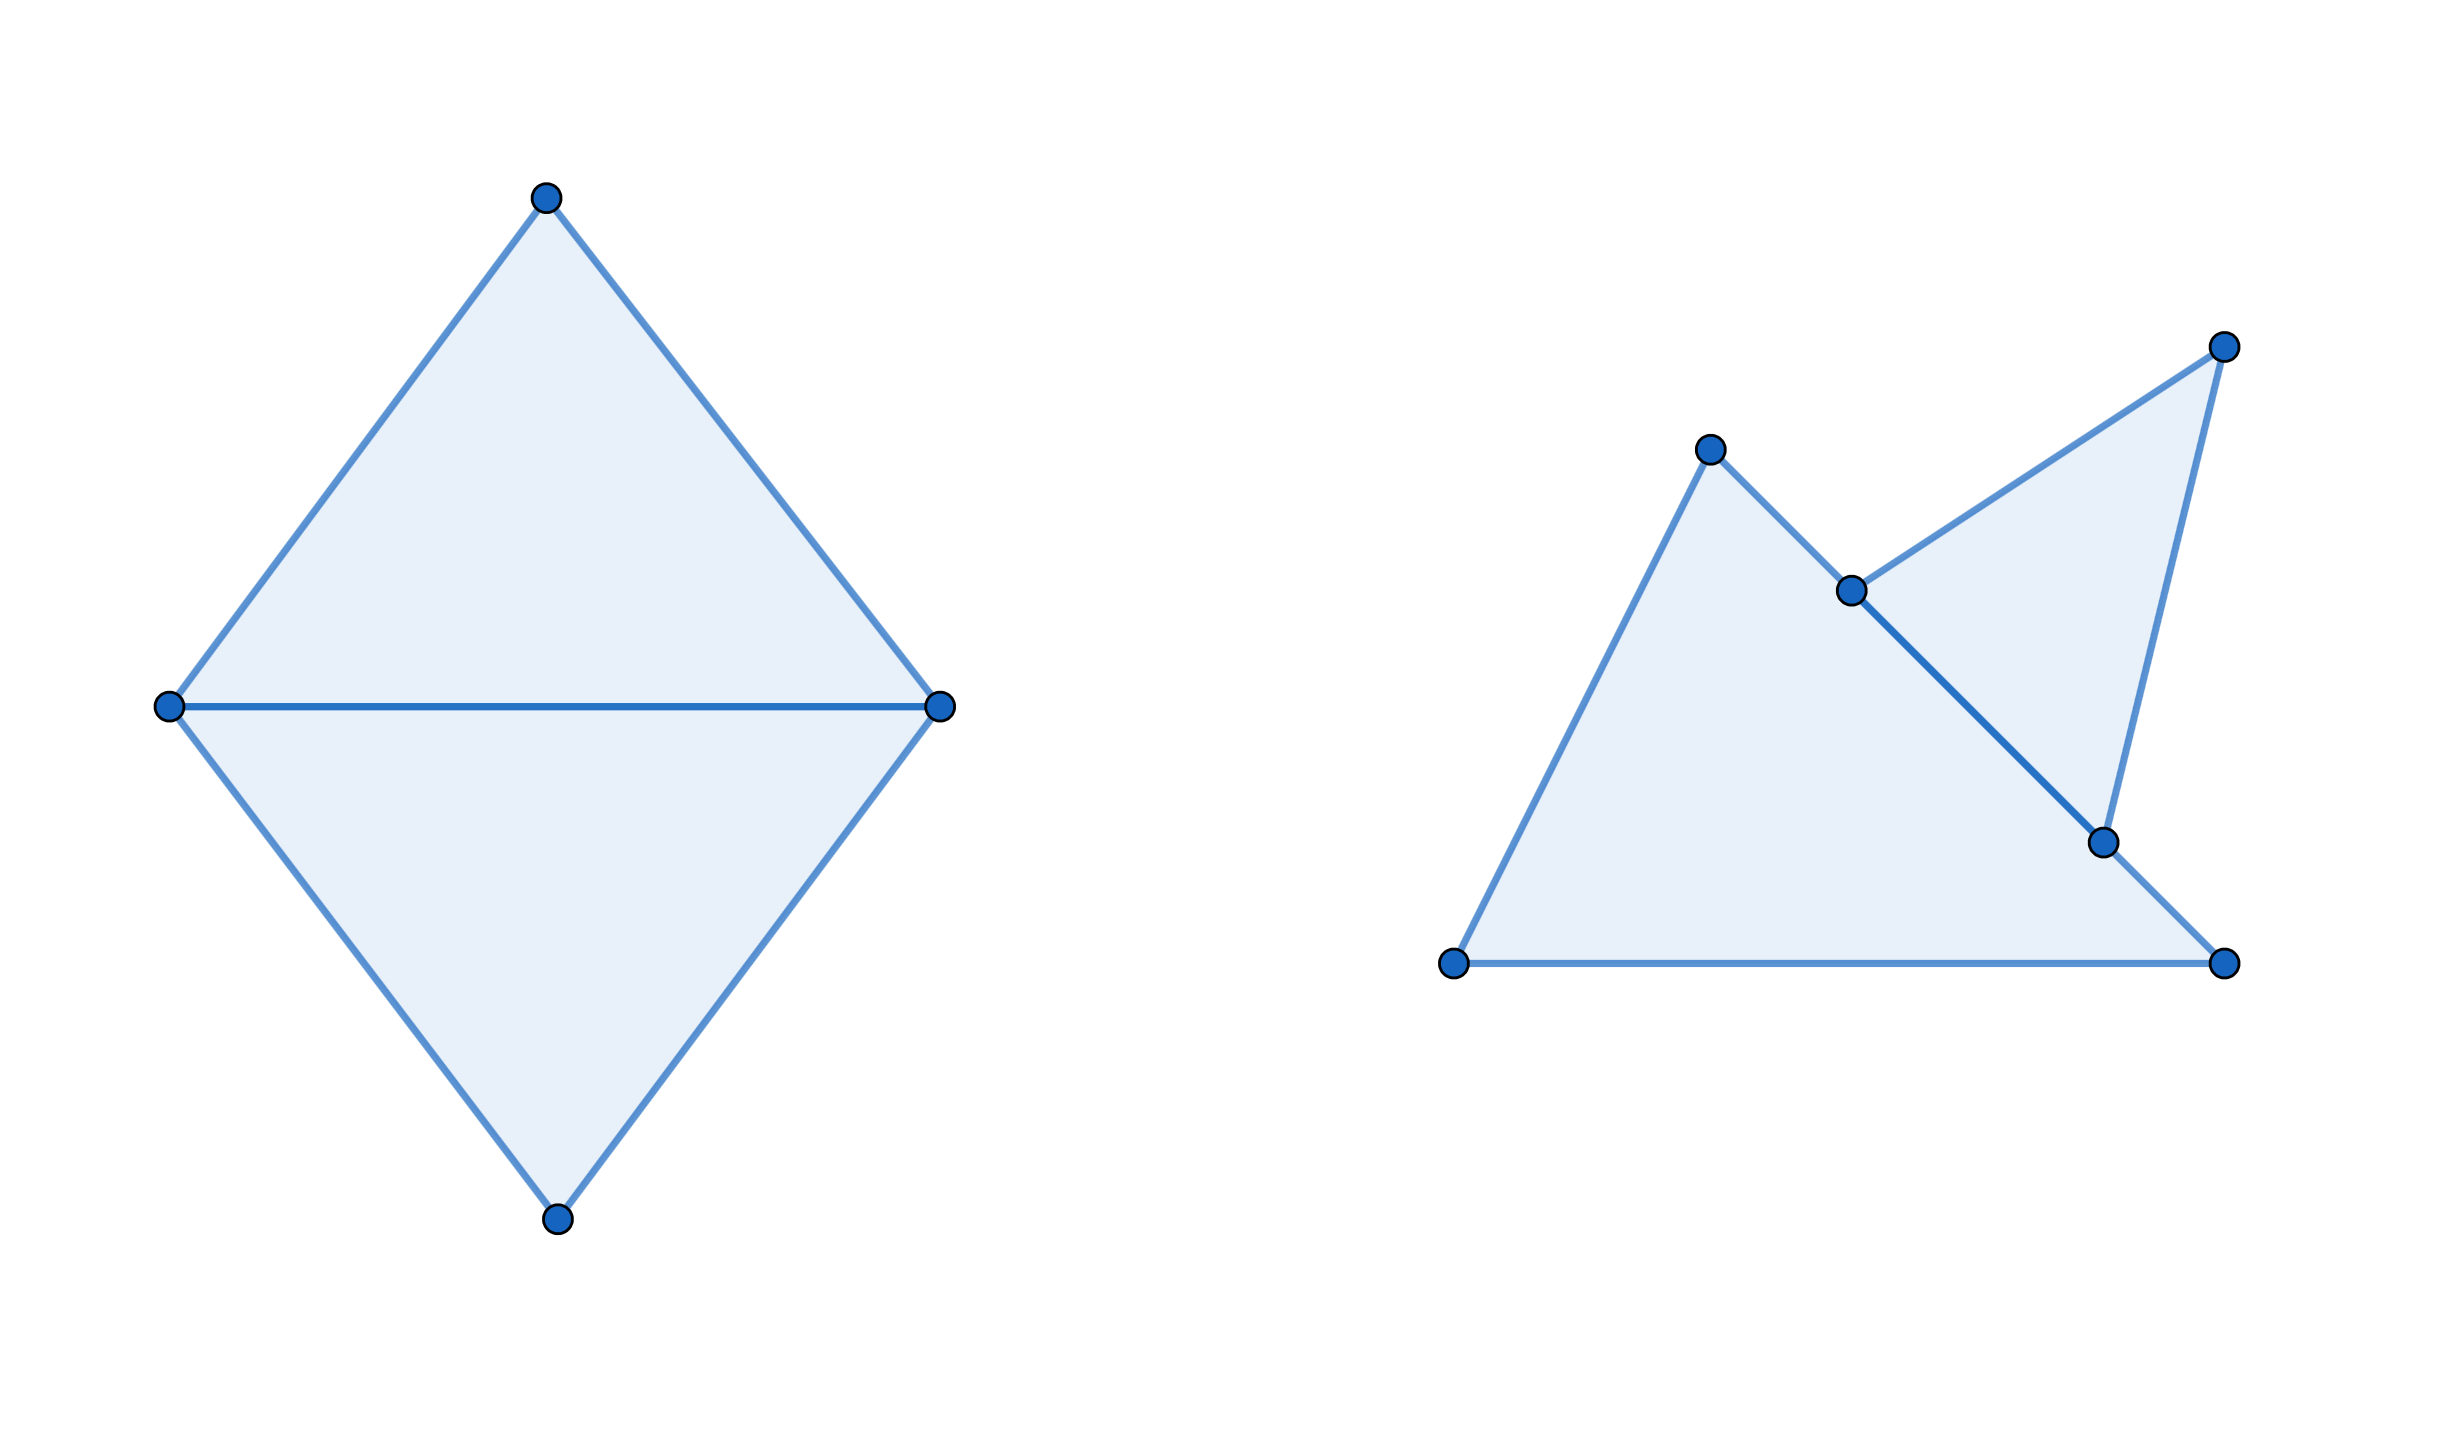
\includegraphics[scale=1.5]{Figures/cell complex_vs_not_cell_complex.png}
\centering
\caption{An example of a $2$-simplicial complex (left) and a not simplicial complex (right).}
\label{fig: sim_comp_example}
\end{figure}

We now introduce some operative definitions that we are going to use in the following sections.

\begin{Def}
    A \textbf{well-centered simplicial complex} is a simplicial cell-complex where the circumcenter of any $p$-simplex of the complex lies in its interior.
\end{Def}

We will require that each $p$-cell is oriented and the orientation is specified by the order of nodes used to represent the $p$-cell. See p. 42-44 of \cite{grady2010discrete} for more details in this regard. 

\begin{Def}
     We also introduce the following notation for $p$-simplices: $\sigma^q \prec \sigma^p$ if and only if $\sigma^q$ is a proper face of $\sigma^p$.
\end{Def}

\begin{Def}
        The \textbf{incidence matrix} $\mathsf{A}_p$ is the matrix which encodes which $p$-cells are incident to which $(p-1)$-cells in the $n$-complex and it is defined as
        \begin{equation}
            \mathsf{A}_p(i,j) = \begin{cases}
                0 \quad \text{if } \sigma^{p-1}_i \text{ is not on the boundary of } \sigma_j^p,\\
                +1 \quad \text{if } \sigma^{p-1}_i \text{ is coherent with the induced orientation of } \sigma^p_j,\\
                -1 \quad \text{if } \sigma^{p-1}_i \text{ is not coherent with the induced orientation of } \sigma^p_j.\\
        \end{cases}
        \end{equation}
\end{Def}

\begin{figure}[t!]
    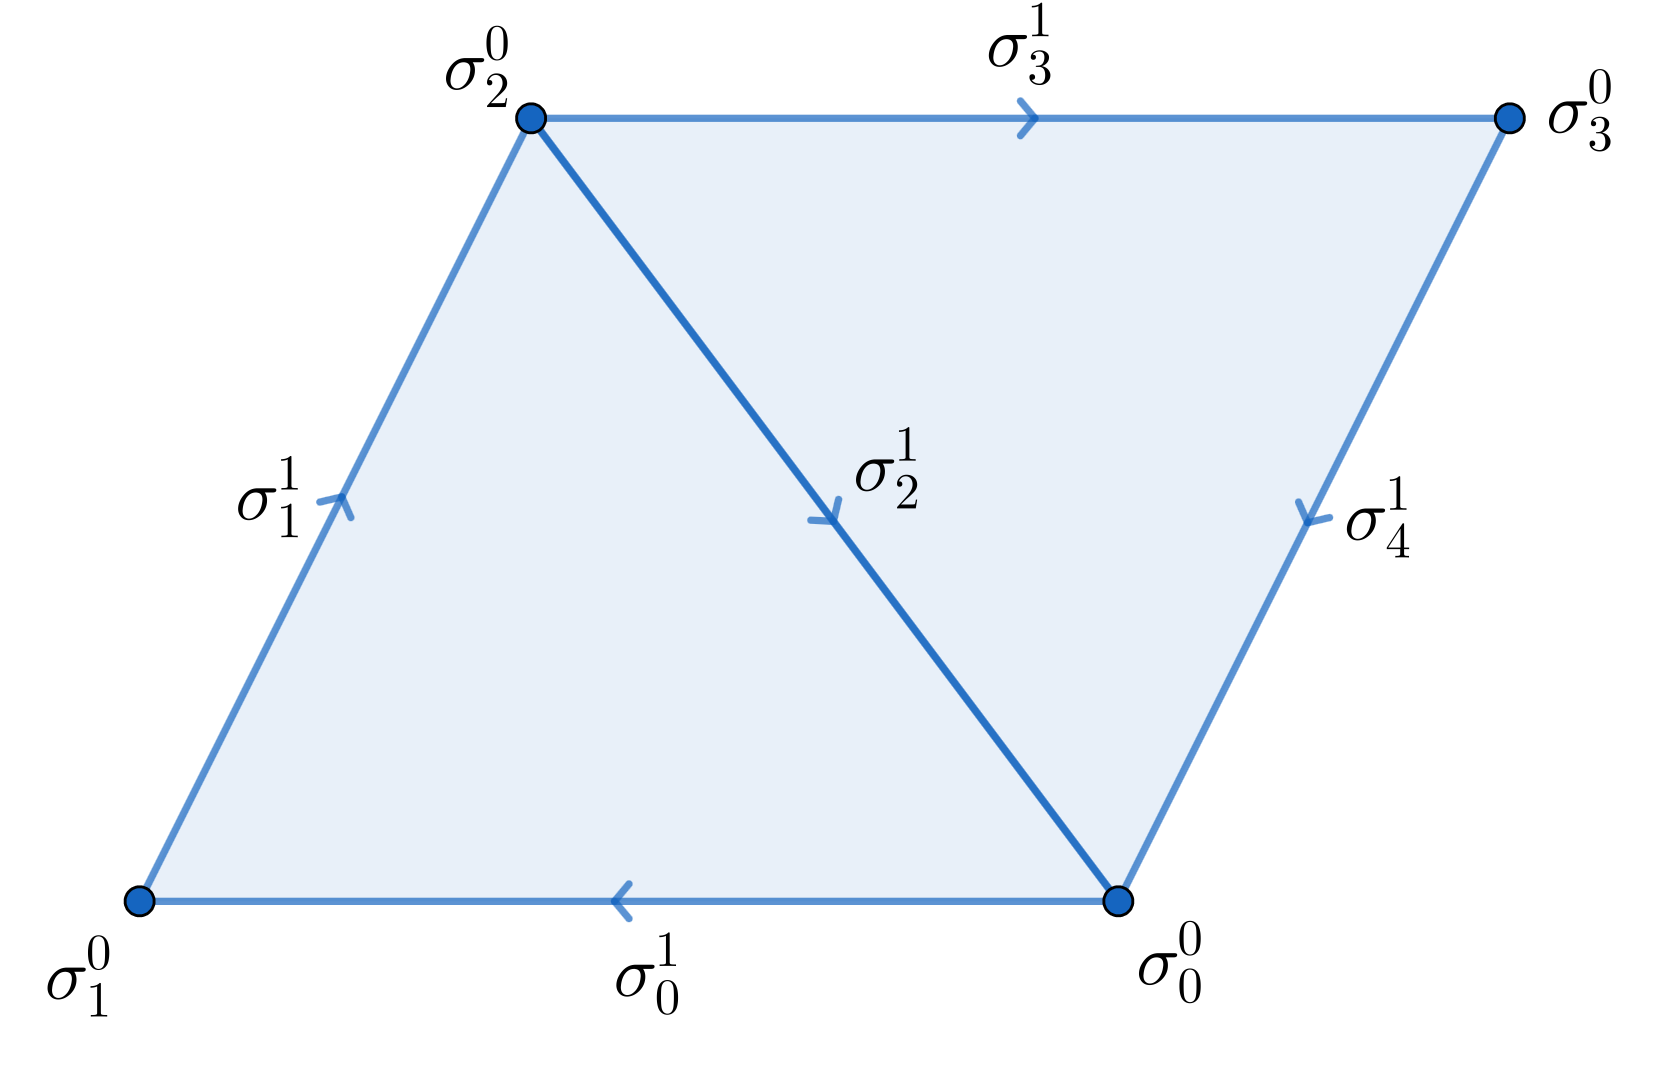
\includegraphics[width=8cm,height=5cm]{Figures/Oriented.png}
    \centering
    \caption{The $2$-simplicial complex of Example~\ref{ex: inc_matrix}.} 
    \label{fig: incidence_matrix}
\end{figure}

\begin{Ex}
    \label{ex: inc_matrix}
    Let us see an explicit example to understand better the previous definition of incidence matrix. Consider the simplicial complex in Figure~\ref{fig: incidence_matrix}.
    In this case, the incidence matrix $\mathsf{A}_1$ is
    \begin{equation*}
        \mathsf{A}_1 = \begin{bmatrix}
            -1 & 0 & 1 & 0 & 1\\
            1 & -1 & 0 & 0 & 0\\
            0 & 1 & -1 & -1 & 0\\
            0 & 0 & 0 & 1 & -1\\
        \end{bmatrix}
    \end{equation*}
\end{Ex}

\begin{Def}
        Let $K$ be a cell complex. A \textbf{$p$-chain} is an $n_p$-tuple of scalars which assigns a coefficient to each $p$-cell, where $n_p$ is the number of distinct $p$-cells in the complex. Each $p$-cell is referred to a \textbf{basic chain}. The $p$-chains group is denoted by $\mathcal{C}_p(K, \rr)$.
\end{Def}

A $p$-chain $c_p$ can be expressed with respect to basic chains:
\begin{equation}
    c_p = \sum_j c_p(\sigma^p_j) \sigma^p_j,
\end{equation}
where $c_p(\sigma^p_j) \in \rr$ and $\sigma^p_j$ is a basic chain for any $j$. Thus, any $p$-chain may be represent by a $n_p \times 1$ (row) vector $\mathsf{c}_p$. By applying the incidence matrix $\mathsf{A}_p$ to $\mathsf{c}_p$ we obtain a $(p-1)$-chain, \textit{i.e.}, in components
\begin{equation}
    \mathsf{c}_{p-1} = \mathsf{A}_p \mathsf{c}_p,
\end{equation}
where $\mathsf{c}_{p-1}$ is the array of the coefficients of the \textbf{boundary} of the $p$-chain $c_p$. Hence, $\mathsf{A}_p$ may be viewed as the matrix representation of the \textbf{discrete boundary operator}. We will indicate the boundary operator with the symbol $\partial$.
Hence, the incidence matrix provides both a representation of the topology of the manifold and a representation of the boundary operator.

Geometrically, $p$-chains are the discrete representation of $p$-vectors: their coefficients (weights) can be used to encode length, areas, etc.
For instance, the $1$-chains represent lengths, while the $2$-chains represent areas and so on.

\subsection{Discrete Forms and Coboundary}

\begin{Def}
        A $p$-\textbf{cochain}, or discrete form, is a linear functional that maps chains to scalars. As for the chains, we can represent cochains in terms of \textbf{basic cochains}
        \begin{equation}
            c^p = \sum_i c^p(\sigma_p^i) \sigma_p^i, \label{eq: cochain_def}
        \end{equation}
        where $a_i \in \rr$ and $\sigma_p^i$ is a basic $p$-cochain. The space of $p$-cochains on a simplicial complex $K$ is denoted by $\mathcal{C}^p(K, \rr)$.
\end{Def}
Cochains, or \textsl{discrete forms}, serve as the discrete analogue of differential forms, and in physical theories they represent discrete fields defined on the elements of a cell complex. Indeed, we know \cite{grady2010discrete} that differential $p$-forms are built taking the dual of the vector space of $p$-vectors and similarly the space of scalar-valued $p$-cochains is the dual of the space of scalar-valued $p$-chains.
We can represent a $p$-cochain as a $1 \times n_p$ (column) vector.

\begin{Def}
        We can define a discrete analogue of \textbf{integration} as the pairing of a $p$-chain with a $p$-cochain, precisely
        \begin{equation}
            \llangle c^p, c_p \rrangle := \sum_{i=1}^{n_p} c_p(\sigma^p_i)c^p(\sigma_p^i).
        \end{equation}
\end{Def}

\begin{Def}
    We define the matrix form of \textbf{coboundary operator} $\mathsf{D}_p$ as the adjoint of the boundary operator through the pairing defined previously, i.e. by definition
    \begin{equation}
        \llangle \mathsf{D}_p\mathsf{c}^{p-1}, \mathsf{c}_p \rrangle = \llangle \mathsf{c}^{p-1}, \mathsf{A}_p\mathsf{c}_p \rrangle.
    \end{equation}
    Hence, $\mathsf{D}_p = \mathsf{A}^T_p$.
    
    Without using components, the coboundary is defined so as to satisfy the (discrete) \textbf{Stokes Theorem}, \textsl{i.e.}, 
    \begin{equation}
        \llangle d c^{p-1}, c_p \rrangle = \llangle c^{p-1}, \partial c_p \rrangle. \label{eq: discrete_Stokes}
    \end{equation}
    
    The \textbf{coboundary operator} (not in components) will be denoted with $d$.
\end{Def}

The coboundary operator can be seen as the discrete counterpart of the exterior derivative, since if we apply the coboundary operator to a $p$-cochain we obtain a $(p+1)$-cochain.

\subsection{Primal and Dual Complexes}
\label{sec: primal_dual_complexes}
To illustrate the necessity of a dual complex in the DEC framework, we consider an example adapted from \cite{tonti2013mathematical}. In the differential formulation of physical laws, operators such as the Laplacian act on functions to express relationships between physical quantities. For instance, the Poisson’s equation
\begin{equation}
    \Delta u(\mathbf{x}) + f(\mathbf{x}) = 0
\end{equation}
relates the source $f$ at $\mathbf{x}$ to the Laplacian of $u$ at the same point. While this might appear to be a purely pointwise relation, it is not truly local: computing the Laplacian at $\mathbf{x}$ involves evaluating derivatives, which depend on a neighborhood of $\mathbf{x}$. In other words, a differential operator inherently requires information from an extended region around each point, whose precise size is not specified. These observations naturally motivate the introduction of an auxiliary structure surrounding the original complex. Collectively, the auxiliary regions associated with each cell form a new complex, known as the \textbf{dual complex}, which provides a discrete representation of these neighborhood interactions in the framework of DEC.

Given a cell complex of dimension $n$, we can define its \textsl{dual} by associating a $p$-cell with an $(n-p)$-cell, following a specific rule. In the case of simplicial complex, the following rules are of relevant importance, since they are the most used in applications.
\begin{itemize}
    \item \textbf{Circumcentric (Voronoi) dual}. Voronoi cells are polygons whose sides are the axes of the edges of a primal simplicial complex.
    \item \textbf{Barycentric dual}. Barycentric cells are polygons obtained by connecting the barycentre of every triangle with the midpoint of the edges of the triangles.
\end{itemize}

For more details on this construction, see section 4.2 of \cite{tonti2013mathematical}. From now on, the circumcentric rule is used to construct the dual complex.

The dual of a cell complex $K$ is indicated as $\star K$ and a generic dual $p$-cell of $\star K$ is indicated as $\star \sigma_{(n-p)}$.

\subsubsection{Orientations}

Once a primal complex is defined, we have to orient it in order to compute properly the boundary matrices. To do so, we choose one of the two possible orientations, clockwise or counterclockwise, for all the $n$-cells and this choice induces an orientation for all the $p$-cells with $0 < p \leq n-1$, see, \textsl{e.g.}, Definition 2.3.5. of \cite{hirani2003discrete}. 
Following \cite{hirani2003discrete}, we do not assign any orientation to points ($0$-cells), even though in \cite{tonti2013mathematical} points are oriented as sinks or sources.

Following this receipt, we can give an orientation to every $p$-cell of the primal complex. This induces an orientation to all the dual $p$-cells, since the primal $p$-cells and dual $(n-p)$-cells have a clear association with each other.
Precisely, following the algorithm described in Remark 2.5.1 of \cite{hirani2003discrete} we are able to orient all the dual $p$-cells.
%Geometrically, for $n=2$ we orient the dual $(n-p)$-cell rotating of $\pi/2$ counterclockwise the orientation of the corresponding primal $p$-cell \cite{crane2018discrete}.

We follow the previous rule to orient primal and dual complex.
Note that this choice is crucial: if we change the orientation rule, we will also have to modify the definition of the DEC operators (coboundary, Hodge star, etc). For example, in \cite{grady2010discrete} the induced orientation of the dual complex is different and consequently the definitions of some operators are slightly different.

\subsubsection{Dual boundary and coboundary}

We wish to define the dual boundary $\partial^{\star}$ in order to also have a dual coboundary $d^\star$ obtained by the relation
\begin{equation}
    \llangle d^\star \alpha, \star \beta \rrangle = \llangle \alpha, \partial^\star  \!\beta \rrangle.
\end{equation}
We have to take care about the sign of the dual boundary, as stated in \cite{schulz2020convergence}. The following definition \cite{schulz2020convergence} is consistent with our orientation rule.

\begin{Def}
        The \textbf{dual boundary operator} $\partial_p^*: \mathcal{C}_p(\star K, \rr) \rightarrow \mathcal{C}_{p-1}(\star K, \rr)$ is the linear operator such that
        \begin{equation}
            \partial_p^\star \star\!\tau = (-1)^{p+1} \sum_{\eta \succ \tau} \star \eta,
        \end{equation}
        where $\star \tau$ is an arbitrary dual $p$-simplex and $\eta$ is a dual $(p+1)$-simplex oriented in order to induce a consistent orientation on $\tau$.
\end{Def}

As we stated previously, the definition of the dual coboundary operator is straightforward now. The following result \cite{munkres2018elements, milicchio2008codimension}, called \textsl{Poincar\`e duality}, gives us an explicit relation between primal coboundary and dual boundary.

 \begin{Th}
        There exists a family of isomorphisms $\phi_p: \mathcal{C}^{p}(K, \rr) \rightarrow \mathcal{C}_{n-p}(\star K, \rr)$ such that the following diagram commutes for any $k$.
        $$\begin{CD}
        \mathcal{C}^{p-1}(K, \rr)   @>\phi_{p-1}>>   \mathcal{C}_{n-p+1}(\star K, \rr)\\
        @VVd_{p-1}V       @VV\partial_{n-p+1}^\star V\\
        \mathcal{C}^{p}(K, \rr)   @>\phi_p>>   \mathcal{C}_{n-p}(\star K, \rr)\\
        \end{CD}$$
\end{Th}

The proof of the previous Theorem (see proof of Theorem 65.1 of \cite{munkres2018elements}) is constructive and we can see that the definition of $\phi_p$ is dependent on the orientation. 

The following result is a practical consequence of the previous statements \cite{schulz2020convergence, desbrun2005discrete}.

\begin{Th}
     Given a primal $n$-complex, the matrix representation of the boundary operator on primal $p$-cells $\mathsf{A}_p$ is the transpose of the (matrix representation of the) boundary operator on dual $(n - p - 1)$-cells ${\mathsf{A}^*_{n-p-1}}$, \textit{i.e.}
     \begin{equation}
         \mathsf{A}_p = (-1)^{p+1}( {\mathsf{A}^{\star}_{n-p-1}})^T,
     \end{equation}
     or equivalently
     \begin{equation}
         \mathsf{A}^\star_{n-p-1} = (-1)^{p+1} \mathsf{A}^T_p
     \end{equation}
\end{Th}

All these relations can be summarized by the following diagram, in which $\star$ is the \textbf{discrete Hodge star} (introduced formally in the next section) which allows us to pass from a primal $p$-cell to its correspondent dual $(n-p)$-cell.

$$\begin{CD}
\mathcal{C}^p(K, \rr)   @>d_p>>   \mathcal{C}^{p+1}(K, \rr)\\
@VV\star_pV       @VV\star_{p+1}V\\
\mathcal{C}^{n-p}(\star K, \rr)   @<d_{n-p-1}^\star = (-1)^{p+1}d^t_p<<   \mathcal{C}^{n-p-1}(\star K, \rr)\\
\end{CD}$$

\begin{Ex}
    To get in touch with the relation between primal and dual coboundary, consider the following example (Figure \ref{orient}).

    \begin{figure}[t!]
    
\includegraphics[scale=1.5]{Figures/Orient.png}
    \centering
    \caption{Primal cell complex (grey) and its dual (blue). Primal $2$-cells are oriented counterclockwise, inducing an orientation on the 1-cells that are not shared by any 2-cell. The dual complex is oriented following the algorithm described in Remark 2.5.1 in \cite{hirani2003discrete}. We remark that the orientation of each oriented dual edge can be obtained by rotating of $\pi/2$ counterclockwise the corresponding primal edge \cite{crane2018discrete}.} 
    \label{orient}
    \end{figure}

    We first orient ever primal $2$-cell counterclockwise, while every primal $1$-cell inherits the orientation of the parent $2$-cell (according to Definition 2.3.5 in \cite{hirani2003discrete}), except $\sigma^1_4$, in which we choose an arbitrary orientation. Now we are able to orient the dual $1$ and $2$-cells \textsl{consistently} with respect to primal orientations. We follow the algorithm described in Remark 2.5.1 in \cite{hirani2003discrete}. To see how it works, we orient for example the dual $2$-cell $\star \sigma^0_0$ and the dual $1$-cell $\star \sigma^1_1$. 
    \begin{enumerate}
        \item We have to understand if $\star \sigma^0_0$ is oriented counterclockwise or clockwise. To do so, following \cite{hirani2003discrete} and his notation we have to compute $$s := \text{sgn}([c(\sigma^0_0), c(\sigma^0_1), c(\sigma^0_2)], \sigma^0_2)$$
        A simple computation shows that $s = 1$, thus the dual simplex $\star \sigma^0_0$ is oriented counterclockwise. Indeed, we have that $\star \sigma^0_0 = s [c(\sigma^0_0), c(\sigma^0_1), c(\sigma^0_2)] = [c(\sigma^0_0), c(\sigma^0_1), c(\sigma^0_2)]$.
        \item For sure $\star \sigma_1^1 = s [c(\sigma^0_1), c(\sigma^0_2)]$, where $s = \pm 1$. According to Remark 2.5.1 of \cite{hirani2003discrete}, we actually have
        $$s = \text{sgn}([c(\sigma^0_0), c(\sigma^0_1)], \sigma^0_1) \cdot \text{sgn}([c(\sigma^0_0), c(\sigma^0_1), c(\sigma^0_2)], \sigma^0_2) = 1\cdot 1 = 1.$$
        Hence, $\star \sigma^1_1 = [c(\sigma^0_1), c(\sigma^0_2)]$.
    \end{enumerate}
    This algorithm gives us an orientation of the dual complex. In this way, we can compute the boundary primal matrix $\mathsf{A}_1$ and the boundary dual matrix $\mathsf{A}^\star_2$. Following the definition of boundary, we get
    \begin{equation*}
        \mathsf{A}_1 = \begin{bmatrix}
            -1 & 0 & 0 & 1 & 0\\
            1 & -1 & 0 & 0 & -1\\
            0 & 1 & -1 & 0 & 0\\
            0 & 0 & 1 & -1 & 1\\
        \end{bmatrix}, \quad 
        \star \mathsf{A}_2 = \begin{bmatrix}
            1 & -1 & 0& 0\\
            0 & 1 & -1 & 0\\
            0 & 0 & 1 & -1\\
            -1 & 0 & 0 & 1\\
            0 & 1 & 0 & -1\\
        \end{bmatrix}.
    \end{equation*}
    Hence, we have $ \mathsf{A}^\star_2 = - \mathsf{A}^T_1$.
    
\end{Ex}

\subsection{The Discrete Hodge Star}

\begin{figure}[t!]
    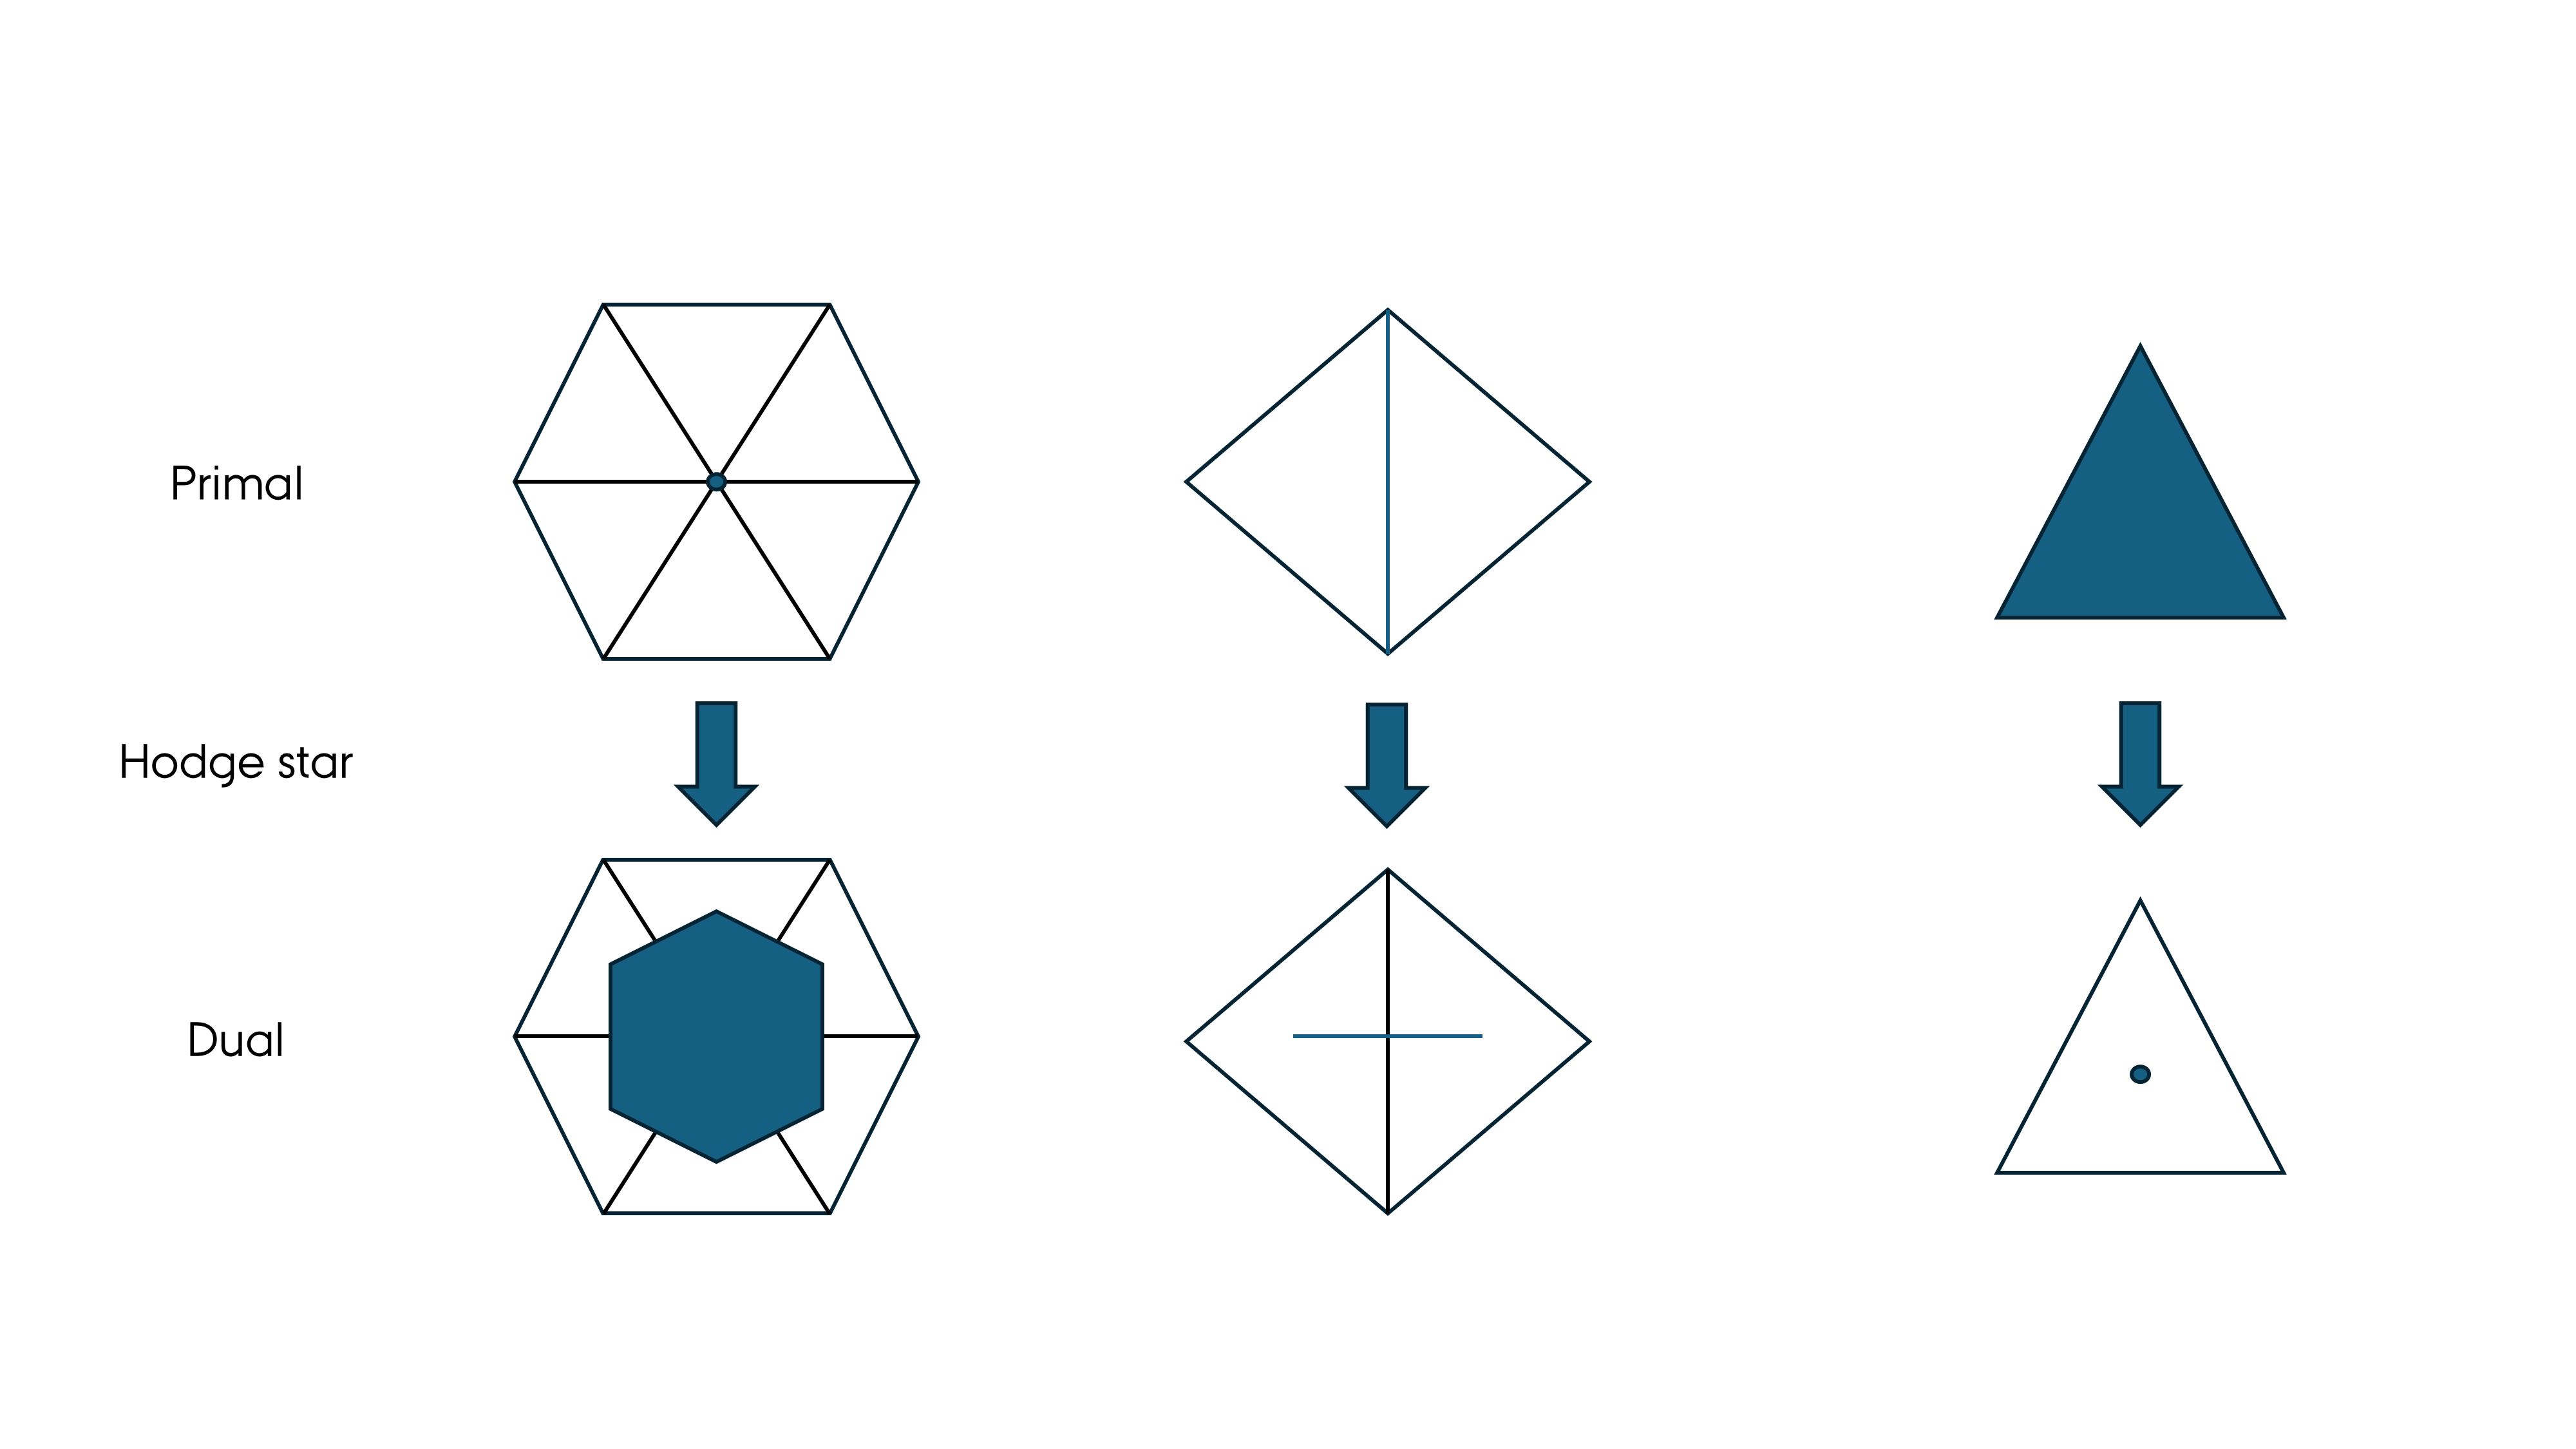
\includegraphics[scale=0.4]{Figures/hodge_star.png}
    \centering
    \caption{The action of the Hodge star.} 
    \label{fig: hodge_star}
    \end{figure}


The continuous Hodge star is an isomorphism between $p$-forms and $(n-p)$-forms. Similarly, in the discrete setting it is an isomorphism between primal $p$-cochains and dual $(n-p)$-cochains.

\begin{Def}
    The \textbf{discrete Hodge star} is the map $\star: \mathcal{C}^p(K, \rr) \rightarrow \mathcal{C}^{n-p}(\star K, \rr)$ defined by the following relation: for any $p$-cochain $c^p$ and $p$-simplex $\sigma_p$
    \begin{equation}
        \frac{1}{|\sigma_p|} \llangle c^p, \sigma_p \rrangle = \frac{1}{|\star \sigma_p|} \llangle \star c^p, \star\sigma_p \rrangle,
    \end{equation}
    where $\star\sigma_p$ is the (only) dual $(n-p)$-simplex corresponding to $\sigma_p$, and $|\sigma_p|$ (respectively $|\star\sigma_p|$) is the volume of the primal $p$-simplex (respectively dual $(n-p)$-simplex).
\end{Def}

As in the continuous theory, the following relation holds \cite{grinspun2006discrete}:
\begin{equation}
    \star_p \star_{n-p} = (-1)^{p(n-p)} \text{Id},
\end{equation}
where, with a slight abuse of notation, we use the symbol $\star$ both for the Hodge star and its inverse. In Figure~\ref{fig: hodge_star} (inspired from the first figure of Section 4.8.4 in \cite{crane2018discrete}) we show graphically the action of this map in some simple cases.

We can now easily translate the definition of the $L^2$ inner product in the discrete setting.

\begin{Def}
    Let $c_1^p, c^p_2 \in \mathcal{C}^p(K, \rr)$, their \textbf{discrete $L^2$ inner product} is defined as 
        \begin{equation}
            \langle c_1^p, c_2^{p} \rangle := \sum_{\sigma^p \in K} \llangle c_1^p, \sigma^p \rrangle \llangle \star c_2^{p}, \star \sigma^p \rrangle \label{innprod}
        \end{equation}
\end{Def}

In matrix-vector form the previous definition becomes
\begin{equation}
    \mathsf{c}^T_1 \mathsf{S} \mathsf{c}_2.
\end{equation}

In the same fashion, it is possible to define the discrete $L^2$ inner product for dual $p$-cochains.

In \cite{desbrun2005discrete} the discrete $L^2$ inner product of $c_1^p, c^p_2 \in \mathcal{C}^p(K, \rr)$ is defined as 
\begin{equation}
    \langle c_1^p, c_2^{p} \rangle := \sum_{\sigma^p \in K} \frac{|V_{\sigma^p}|}{|\sigma^p||\star \sigma^p|} \llangle c_1^p, \sigma^p \rrangle \llangle \star c_2^{p}, \star \sigma^p \rrangle = \frac{1}{n} \sum_{\sigma^p \in K} \llangle c_1^p, \sigma^p \rrangle \llangle \star c_2^{p}, \star \sigma^p \rrangle,
\end{equation}
which becomes in matrix-vector form
\begin{equation}
    \frac{1}{n}\mathsf{c}^T_1 \mathsf{S} \mathsf{c}_2.
\end{equation}

We prefer to define the discrete inner product as in \eqref{innprod}. Indeed, ``mimicking the smooth setting, each inner product matrix $\mathsf{S}$ determines a linear mapping from a discrete
$p$-form to a discrete version of the dual $(n-p)$-form'' (hence a discrete Hodge star operator!) \cite{de2016subdivision}. In other words, the second definition is not consistent with our definition of the Hodge Star since, for $n \neq 1$, $\frac{1}{n} \mathsf{S} \neq \mathsf{S}$.

\subsection{The Discrete Laplace-de Rham Operator}
To define the discrete version of the Laplace-de Rham Operator we need the concept of discrete codifferential, following the derivation obtained in the continuos setting.

 \begin{Def}
        The \textbf{discrete codifferential operator} $\delta_p$ maps \textsl{primal} $p$-cochains into \textsl{primal} $(p-1)$-cochains via a mapping into the \textsl{dual} complex and is defined as
        \begin{equation}
            \delta_p := (-1)^{n(p-1) + 1} \star d^\star_{n-p} \star.
        \end{equation}

        Moreover, by definition $\delta_0 \equiv 0$.
\end{Def}

In the previous definition, we write $\star$ both for primal to dual map and dual to primal map. The definition above is obtained requiring that, for any $\alpha \in \mathcal{C}^{p-1}(K, \rr), \beta \in \mathcal{C}^{p}(K, \rr)$
\begin{equation}
    \langle d\alpha, \beta  \rangle = \langle \alpha, \delta \beta \rangle.
\end{equation}

We can define similarly the discrete dual codifferential operator as a map from dual $p$-cochains to dual $(p-1)$-cochains as follows. We require that for any $\alpha \in \mathcal{C}^{p-1}(\star K, \rr), \beta \in \mathcal{C}^{p}(\star K, \rr)$
\begin{equation}
    \langle d^*\alpha, \beta  \rangle = \langle \alpha, \delta^* \beta \rangle.
\end{equation}
Performing all the computations and exploiting the previous equation we finally get
\begin{equation}
    \delta^*_p := (-1)^{p(n+1-p)} \star d_{n-p} \star.
\end{equation}

\begin{Def}
    The \textbf{discrete Lapalce-de Rham Operator} is defined as
    \begin{equation}
        \Delta := d\delta + \delta d.
    \end{equation}
\end{Def}

\subsection{de Rham Maps and Discrete Flat Operators}
The de Rham maps establish a connection between smooth differential forms and cochains. These maps encode how continuous geometric and physical quantities, such as fields or fluxes, can be integrated over simplices in a simplicial complex.

In the following, let $M$ be a smooth triangulable $n$-manifold and $K$ be a simplicial complex homeomorphic to $M$, as in \cite{hirani2003discrete}. In the following, $\Lambda^p(M)$ is the space of continuous $p$-form on $M$.

\begin{Def}
    The \textbf{de Rham map} is the map $\mathcal{R}^p: \Lambda^p(M) \rightarrow \mathcal{C}^p(K, \rr)$ defined as
     \begin{equation}
         \llangle \mathcal{R}^p(\omega), c_p \rrangle := \sum_i a_i \int_{\sigma^p_i} \omega,
     \end{equation}
     where $c_p = \sum_i a_i \sigma^p_i$ is a generic $p$-chain. The definition of the \textbf{dual de Rham map} is analogous.
\end{Def}


This definition associates to each smooth differential form a discrete cochain by integrating the form over simplices.  In this way, continuous geometric data are transferred into an algebraic setting where they act linearly on chains, providing a natural link between differential and diiscrete forms.

%This is a quite natural definition. Indeed, we have already seen that each continuous $p$-form can be integrated over a $p$-simplex, hence it is straightforward to define its ``cochain counterpart'' as the cochain in which the scalar related to $\sigma^i_p$ is $\int_{\sigma^i_p} \omega$.

To connect discrete data with continuous geometric structures, interpolation operators are used to reconstruct smooth fields from discrete differential forms.


\begin{Def}
    A \textbf{primal interpolation} is a function $\mathcal{I}^1: \mathcal{C}^0(K, \rr) \rightarrow \Lambda^1(M)$ and similarly a \textbf{dual interpolation} is a function $\mathcal{I}^{\star 1}: \mathcal{C}^0(\star K, \rr) \rightarrow \Lambda^1(M)$.
\end{Def}

\begin{Def}
    Given a primal interpolation function $\mathcal{I}^1$, we define the \textbf{discrete primal 1-flat} $\flat_1$ as the function $\flat_1: \mathcal{C}^0(K, \rr) \rightarrow \mathcal{C}^1(K, \rr)$ such that
    \begin{equation}
        \flat_1(c^0) := \mathcal{R}^1(\mathcal{I}^1(c^0)).
    \end{equation}
    The definition of the \textbf{discrete dual 1-flat} is analogous.
\end{Def}

The idea of this definition comes from \cite{hirani2003discrete} and \cite{boom2022geometric}, the difference being that we explicitly separate the contribution of interpolation from the process of integration. We remark that in this definition we are identifying primal/dual $0$-cochains and discrete (one-dimensional) vector fields\footnote{For a formal definition of a discrete vector field, see Definition~5.1.1-5.1.2 in \cite{hirani2003discrete}.}, so that the discrete $1$-flat can be identified as a map between discrete fields and forms (as in the continuous framework).

\begin{Ex}[Some flat operators in 1D]
\label{ex: flat_example}
Consider a 1-simplicial complex $K$ with $m+1$ vertices and $m$ edges. An example with $m=4$ is provided in Figure~\ref{fig: 1_simpl_compl_example}. Let $\{\sigma^0_0, \dots, \sigma^0_m\}$ and $\{\sigma^1_0, \dots, \sigma^1_{m-1}\}$ be respectively the sets of vertices and edges of $K$.
\begin{figure}[t!]
    \centering
    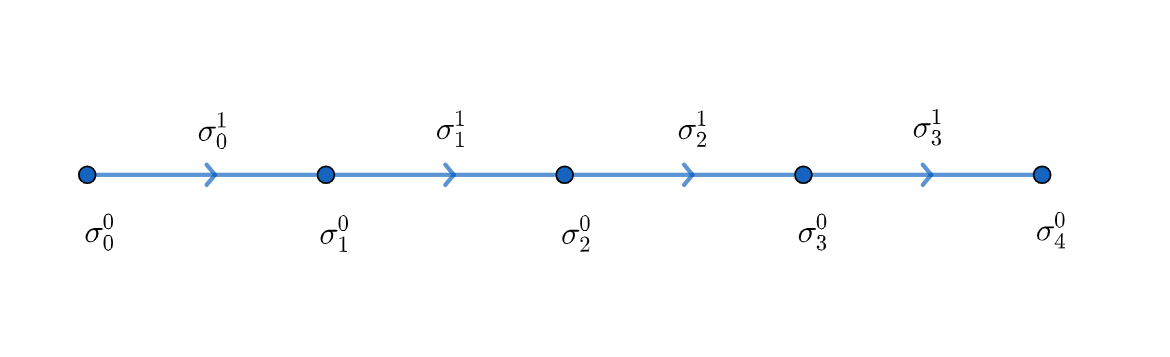
\includegraphics[scale=1.5]{Figures/1_simpl_comp.png}
    \caption{An example for $m=4$ of the 1-simplicial complex considered in Example~\ref{ex: flat_example}.}
    \label{fig: 1_simpl_compl_example}
\end{figure}
Note that in this case, the manifold $M$ can be defined as an open (continuous) interval containing the 1-simplicial complex $K$\footnote{To be precise, this is not rigorous: we are going to define interpolation function that return forms which are differentiable in the interior of each $1$-simplex.}.To keep the notation concise, in this context we will use the same notation for the 0-simplices and its (1D) coordinates.

    \paragraph{Parabolic flat} In this case, we define, for $ x \in (\sigma^0_{i}, \sigma_{i+1}^0),$
    \begin{equation}
        \mathcal{I}^1(c^0) := \bigg ( \frac{c^0(\sigma^{i+1}_0) - c^0(\sigma^{i}_0)}{\sigma_{i+1}^0 - \sigma_{i}^0} x  + c^0(\sigma^{i}_0) -  \frac{c^0(\sigma^{i+1}_0) - c^0(\sigma^{i}_0)}{\sigma_{i+1}^0 - \sigma_{i}^0} \bigg ) \mathrm{d} x, 
    \end{equation}
    using the notation introduced in \eqref{eq: cochain_def}. Thus, we have
    \begin{align}
        \flat^1_{\text{par}}(c^0)(\sigma^i_1) &= \int_{\sigma^1_i} \mathcal{I}^1(c^0)\\
        &= \int_{\sigma_{i}^0}^{\sigma_{i+1}^0} \bigg ( \frac{c^0(\sigma^{i+1}_0) - c^0(\sigma^{i}_0)}{\sigma_{i+1}^0 - \sigma_{i}^0} x  + c^0(\sigma^{i}_0) -  \frac{c^0(\sigma^{i+1}_0) - c^0(\sigma^{i}_0)}{\sigma_{i+1}^0 - \sigma_{i}^0} \bigg ) \mathrm{d} x\\
        & = \frac{c^0(\sigma^{i}_0) + c^0(\sigma^{i+1}_0)}{2} (\sigma_{i+1}^0 - \sigma_{i}^0).
    \end{align}
    
    \paragraph{Downwind flat} We define for $ x \in (\sigma_{i}^0, \sigma_{i+1}^0),$
    \begin{equation}
        \mathcal{I}^1(c^0) := c^0(\sigma^{i+1}_0) dx,
    \end{equation}
    which gives
    \begin{equation}
        \flat^1_{\text{dow}}(c^0)(\sigma^i_1)= \int_{\sigma^1_i} \mathcal{I}^1(c^0) = c^0(\sigma^{i+1}_0)(\sigma_{i+1}^0 - \sigma_{i}^0).
    \end{equation}
    
    \paragraph{Upwind flat} Similarly, we define for $ x \in (\sigma_{i}^0, \sigma_{i+1}^0),$
    \begin{equation}
        \mathcal{I}^1(c^0) := c^0(\sigma^{i}_0) dx,
    \end{equation}
    which gives
    \begin{equation}
        \flat^1_{\text{upw}}(c^0)(\sigma^i_1)= \int_{\sigma^1_i} \mathcal{I}^1(c^0) = c^0(\sigma^{i}_0)(\sigma_{i+1}^0 - \sigma_{i}^0).
    \end{equation}
\end{Ex}

\subsection{Vector-Valued Cochains}

Until now, greater attention was given to the discrete counterpart of scalar differential forms. However, in the continuous setting we frequently face cases where we have to manipulate vector and tensor fields. Thus, we need to translate this framework properly in the discrete scenario.
 In other words, a generalization of the definition of cochain is needed.

 \begin{Def}
        A \textbf{vector-valued $p$-cochain} is the group of linear functions from $\mathcal{C}_p(K, \rr)$ to a vector space $V$ and it is indicated as $\mathcal{C}^p(K, V)$. In the same fashion,  let Lin be the vector space of tensors. A \textbf{tensor-valued $p$-cochain} is the group of linear functions from $\mathcal{C}_p(K, \rr)$ to Lin and it is indicated as $\mathcal{C}^p(K, \text{Lin})$.
\end{Def}

Any vector-valued $p$-cochain can be written as a linear combination (with vector coefficients!) of basic $p$-cochains, \textsl{i.e.}, we can write a generic vector-valued $p$-cochain as
\begin{equation}
    \mathbf{c}^p = \sum_i \cc^p(\sigma_p^i)\sigma_p^i,
\end{equation}
where each $\cc^p(\sigma_p^i) \in \mathcal{V}$.

Reasoning in components, let $\{\ee_1, \dots, \ee_n\}$ be a base of a vector space $V$. A vector valued $p$-cochain $\cc^p$ maps a $p$-chain $c_p$ into a vector $\cc^p(c_p) = \cc^p_i \ee_i$. Note that $\cc^p_i$ is a linear map from $p$-chains to scalars, i.e. a scalar-valued $p$-cochain! 
An analogous analysis can be done for tensor-valued cochains.

Notice that all the discrete theory developed so far should be properly extended in this case. Some operations are straightforward to extend (\textsl{e.g.}, the inner product), but for others an extended differential theory is needed.
For example, the coboundary of vector valued-cochains can be seen as the discrete version of the exterior covariant derivative \cite{berwick2021discrete}.
Since not all the operators will be of our interest for vector-valued cochains, we are not going to present their formal extension here. For further information, we refer the reader to \cite{berwick2021discrete}. 

\section{Application of DEC to Computational Physics: Examples}
\label{sec: dec_examples}

This section presents a series of examples demonstrating the application of DEC to classical problems in computational physics. We showcase how DEC provides a powerful and flexible framework for building the governing equations of several physical systems on discrete manifolds.

\subsection{2D Poisson Equation}
Here, we derive the stationary diffusion equation with source term (\textsl{i.e.}, the \textsl{Poisson Equation}) using the tools of discrete calculus seen in the previous sections. We remark that our formulation is inherently discrete, \textit{i.e.}~we \textsl{do not} discretize the continuous Poisson equation.

In 2D, let us consider a primal 2-complex consisting of $n$ vertices. We assign an orientation of the primal complex and the dual complex as described in Section~\ref{sec: primal_dual_complexes}. In particular, we orient every primal $2$-cell counterclockwise and we find, by applying the algorithm of Remark 2.5.1 in \cite{hirani2003discrete}, that also dual $2$-cell are oriented counterclockwise. A portion of an example of the 2D simplicial complex is represented in Figure~\ref{fig: diffusion_complex}.

\begin{figure}[htb!]%
    \centering
    \includegraphics[width=5.8cm,height=4.5cm]{Figures/DiffusionDual.png}
    \caption{A portion of the 2D simplicial cell complex considered (light blue) and its \textit{circumcentric} dual (red).}
    \label{fig: diffusion_complex}
\end{figure}

We represent the diffusing quantity as a primal (scalar-valued) $0$-cochain denoted by the symbol $u$. Applying the coboundary operator $d_0$ we get a primal scalar-valued $1$-cochain $d_0 u$ in which the scalars attached to every basic $1$-cochain are the discrete equivalent of the gradient of the continuous scalar field integrated along the edge.
To pass from a circulation to a flux across the edges, we apply the Hodge star operator $\star_1$, which provides a scalar-valued dual $1$-cochain $\star_1 d_0 u$. Then, using a linear and isotropic constitutive equation to relate the diffusive flux $h$ to $ \star_1 \, d_0 u$, we write
\begin{equation}
    h = - k \star_1 d_0 u,
\end{equation}
where $k$ is a (constant) material parameter (conductivity/diffusivity). Since the dual $2$-cells are oriented counterclockwise, following \cite{tonti2013mathematical} the positive orientation for $h$ describes the flux \textit{leaving} any dual $2$-cell.

To obtain the \textit{net} flux \textit{entering} any dual $2$-cell we have to add up the contributions along its boundary using the dual coboundary operator $d^\star$ $(= -d^t_0$, see Section 2.3) and then change the sign of the result. If $f$ is a known dual $2$-cochain which describes the external sources of the dual $2$-cells, the balance equation reads
\begin{equation}
    -d^\star h + f = 0.
\end{equation}
Using the constitutive equation for the flux
\begin{equation}
     k \, d^t_0 (\, \star_1 d_0 u) + f = 0. \label{withoutlap}
\end{equation}

To recover the formulation of diffusion equation with discrete Laplacian, recall that
\begin{equation}
    \Delta := \delta d + d\delta.
\end{equation}
Since $u$ is a $0$-cochain, $d \delta u = 0$ by definition of $\delta$. Moreover, since $\delta_1 = - \star d^\star \star$, applying the (inverse of) Hodge star operator (we again write $\star$ both for primal to dual map and dual to primal map) to \eqref{withoutlap} we get 
\begin{equation}
    -k \Delta u + \Tilde{f} = 0,
\end{equation}
where $\Tilde{f} := \star f$. Since the Laplacian acting on fields $\nabla^2$ is minus the Laplacian on forms (see \cite{frankel2011geometry}), the last equation is the discrete analogous of the Poisson equation $k\nabla ^ 2 u + \Tilde{f} = 0 $ (where $u$ and $\Tilde{f}$ are scalar fields).

In the continuous setting, one can show \cite{evans2010partial} that the Poisson equation arises as the stationarity conditions of the Dirichlet functional, which comprises two terms: the first is the $L^2$ norm of the gradient of the unknown field, and the second is the  $L^2$ inner product between the unknown field and the source term. Similarly, in the discrete setting, a discrete Dirichlet energy can be defined by representing the dimensionless unknown $u$ and the source $f$ as primal scalar-valued $0$-cochains: 
\begin{align}
\mathcal{E}_{\text{p}}(u) := \frac{1}{2} \langle du, du \rangle - \langle u, f \rangle = \frac{1}{2} \langle \delta du, u \rangle - \langle u, f \rangle. \label{eq:discDirichlet}
\end{align}
Here, $du$ is the coboundary of $u$, a primal scalar-valued 1-cochain whose entries correspond to the integral of the continuous gradient field along the mesh edges. Consequently, each term in \eqref{eq:discDirichlet} preserves the same physical and geometric interpretation as in the continuous formulation.

\subsection{Euler's Elastica}

In the following, $\mathcal{I} = [0,L]\subset \rr$ is a one-dimensional interval that represents the coordinates of the points of the longitudinal axis of the rod in its undeformed, straight configuration, $L$ is the length of the rod, $u(\sigma)$ is the angle formed by the tangent to the axis of the rod and the horizontal direction at the dimensionless arc-length $\sigma := s/L$.
For a constant cross-section rod subject to a vertical end-load at the right end and clamped at the left end, the boundary-value problem for the (dimensionless) continuous Euler's Elastica equation reads \cite{audoly2000elasticity}
\begin{align}
        \frac{\textrm{d}^2 u}{\textrm{d}\sigma^2} + f \cos u = 0  \quad \text{in } [0,1], \quad u(0) = 0, \quad \frac{\textrm{d}u}{\textrm{d}\sigma}(1) = 0. \label{contElastica}
\end{align}
In ~\eqref{contElastica}, $f = PL^2/B$ is the dimensionless load parameter, where $P<0$ is the vertical component of the load applied at the right end and $B$ is the \textsl{bending stiffness} of the rod.
The variational formulation of ~\eqref{contElastica} is
\begin{equation}
        \min_{u}\ \frac{1}{2}\int_{0}^1 \left(\frac{\textrm{d}u}{\textrm{d}\sigma}\right)^2\,\textrm{d}\sigma - \int_{0}^1 f \sin u  \,\textrm{d}\sigma ,\quad u (0) = 0. \label{contElasticaEnergy}
\end{equation}

To derive the discrete version of ~\eqref{contElastica} and ~\eqref{contElasticaEnergy}, consider a $1$-simplicial complex representing a discrete rod. The discrete elastica energy can be formulated as
% \begin{equation}
%         \mathcal{E}_{\text{el}}(u) := \frac{1}{2} \langle \mathbbm{1}_{\text{int}} \odot \star d^\star u, \star d^\star u \rangle - \langle f\mathbbm{1}, \sin u  \rangle, \label{eq: discElasticaEnergy}
% \end{equation}
\begin{equation}
        \mathcal{E}_{\text{el}}(u) := \frac{1}{2} \langle k, \star d^\star u \rangle - \langle f\mathbbm{1}, \sin u  \rangle, \label{eq: discElasticaEnergy}
\end{equation}
where $\mathbbm{1}$ is the dual one $0$-cochain, $k := \mathbbm{1}_{\text{int}} \odot \star d^\star u$ is the primal $0$-cochain that encodes the (discrete) curvatures on the nodes and $\mathbbm{1}_{\text{int}}$ is the primal $0$-cochain that is identically $1$ on the interior and $0$ on the boundary nodes.
We can re-write ~\eqref{eq: discElasticaEnergy} as
\begin{align}
    \mathcal{E}_{\text{el}}(u) &= \frac{1}{2} \langle \star (\mathbbm{1}_{\text{int}} \odot \star d^\star u), d^\star u \rangle - \langle f\mathbbm{1}, \sin u  \rangle\\
    &= \frac{1}{2} \langle \delta^\star \star (\mathbbm{1}_{\text{int}} \odot \star d^\star u), u \rangle - \langle f\mathbbm{1}, \sin u  \rangle\\
    &= \frac{1}{2} \langle \delta^\star\star k, u \rangle - \langle f\mathbbm{1}, \sin u  \rangle,
\end{align}
Computing the first variation of the discrete functional we get
\begin{equation}
    \delta^\star \star k - f\cos(u) = 0,
\end{equation}
which is equivalent, using the definition of the codifferential, to
\begin{equation}
     -\star d k - f\cos(u) = 0. \label{discElastica}
\end{equation}

\subsection{2D Linear Elasticity}
Let $K$ be a $2$-simplicial complex, $\hat{\mathbf{e}}_i$ be the Cartesian coordinate framework, ${\mathbf{e}}_i$ be the reference local basis of a given $2$-simplex and ${\mathbf{e}'}_i$ be the local basis of the deformed $2$-simplex. The contravariant bases are indicated with upper indexing. Denoting with $\mathbf{F}$ the deformation gradient of a given $2$-simplex we have\footnote{We adopt Einstein notation for brevity.}
\begin{equation}
    \mathbf{F} = {\mathbf{e}'}_i \otimes {\mathbf{e}}^i.\label{eq:  defgrad}
\end{equation}
Indeed, for any $k$ we have
\begin{equation}
    \mathbf{F} \mathbf{e}_k = ({\mathbf{e}'}_i \otimes {\mathbf{e}}^i) \mathbf{e}_k = {\mathbf{e}'}_i ({\mathbf{e}}^i \cdot {\mathbf{e}}_k) = {\mathbf{e}'}_k. 
\end{equation}
Now recall that
\begin{equation}
    {\mathbf{e}'}_i = ({\mathbf{e}'}_i)_j \hat{\mathbf{e}}_j, \quad {\mathbf{e}}_k = ({\mathbf{e}'}_k)_l \hat{\mathbf{e}}_l, \quad \mathbf{e}^i = \mathbf{g}^{ik}_R \mathbf{e}_k,
\end{equation}
where $\mathbf{g}^{ik}_R := \mathbf{e}^i \cdot \mathbf{e}^k$. Putting everything together in \eqref{eq: defgrad} we get
\begin{equation}
    \mathbf{F} = ({\mathbf{e}'}_i)_j \hat{\mathbf{e}}_j \otimes \mathbf{g}^{ik}_R ({\mathbf{e}}_k)_l \hat{\mathbf{e}}_l = ({\mathbf{e}'}_i)_j \mathbf{g}^{ik}_R ({\mathbf{e}}_k)_l \hat{\mathbf{e}}_j \otimes \hat{\mathbf{e}}_l.
\end{equation}
In particular, in matrix notation we have 
\begin{equation}
    \sf{F} = (\sf{A}')^T \sf{g}_R\sf{A},
\end{equation}
where $\sf{A}$ (resp. $\sf{A}'$) is the matrix where the $i$-th rows is the $i$-th basis vector ${\mathbf{e}}_i$ (resp. ${\mathbf{e}'}_i$). 
Thus, we may represent the deformation gradient $\mathbf{F}$ as a dual (tensor-valued) zero-cochain. Now, we define the 2D infinitesimal strain measure as the following dual zero-cochain
\begin{equation}
    \mathbf{E} := \frac{1}{2} (\mathbf{F} + \mathbf{F}^T) - \mathbf{I}, \label{eq: strain}
\end{equation}
where $\mathbf{I}$ is the identity dual zero-cochain.
By applying the constitutive equation for linearly elastic isotropic bodies, we can compute the dimensionless stress as a dual zero-cochain
\begin{equation}
    \mathbf{S} := 2 \mathbf{E} + \frac{\lambda}{\mu} \text{tr}(\mathbf{E})\mathbf{I},
\end{equation}
where $(\mu,\lambda)$ are the Lam\'e moduli. Note that when computing the stress cochain $\mathbf{S}$ we are multiplying (coefficient-wise) a scalar-valued ($\text{tr}(\mathbf{E})$) and a tensor-valued ($\mathbf{I}$) cochain.

In the case of zero body forces and Dirichlet boundary conditions, we easily derive the potential energy as
\begin{equation}
    \mathcal{E}_{\text{LE}} := \frac{1}{2}\langle \mathbf{S}, \mathbf{E} \rangle. \label{eq: en_le_zero_bf}
\end{equation}

In case of non-zero body forces, \eqref{eq: en_le_zero_bf} becomes
\begin{equation}
    \mathcal{E}_{\text{LE}} := \frac{1}{2}\langle \mathbf{S}, \mathbf{E} \rangle - \langle \mathbf{u}, \mathbf{f} \rangle,
\end{equation}
where $\mathbf{u}$ and $\mathbf{f}$ are the primal vector-valued zero cochains representing, respectively, the dimensionless displacements of the primal nodes and the body force at each primal node.

\subsection{Burgers' equation}
\label{sec: dec_fv}
Finite Volume (FV) schemes and DEC share a deep structural connection, as both rely on integral formulations of conservation laws over discrete domains. In FV methods, fluxes are computed across control volume interfaces to ensure local conservation. DEC, on the other hand, provides a coordinate-free framework for discretizing differential forms, naturally encoding fluxes through discrete Stokes’ theorem. This correspondence reveals that many FV schemes can be interpreted as specific realizations of DEC, highlighting their common geometric and conservation principles. In this section, we show this link through an illustrative example, the Burger's equation, which is closely related to the first-order traffic flow models.

In the continuous setting, the general form of the one-dimensional Burgers' equation, also called \textsl{viscous Burgers' equation}, reads
\begin{equation}
	u_t = - uu_x + \nu u_{xx}, \label{eq: viscidburgers}
\end{equation}
where $u(x,t)$ is the speed of fluid in $(x,t)$ and $\nu$ is the viscosity of the fluid. The \textsl{inviscid Burgers' equation} is obtained by setting $\nu = 0$ and it is a prototype for conservation equations that can develop \textsl{shocks}
\begin{equation}
		u_t = -(u^2/2)_x.
\end{equation} 

In the discrete setting, a $1$-simplicial complex models the space, while the time interval is uniformly discretized with step-size $\Delta_t$.
The unknown $U^n$ is the average value of the velocity field at the time $t = n\Delta_t$ in a given dual edge and it is represented as a dual $0$ cochain. The flux $F$ is a primal $0$-cochain such that
\begin{equation*}
	F^n_{i - 1/2} := f(U^n_{i-1}, U^n_i),
\end{equation*}
where $f$ is some numerical flux function (as in the Finite Volume Method schemes). Forward Euler method is chosen to treat the term $u_t$.
The discrete version of the Burgers' equation reads in general 
\begin{equation}
	U^{n+1}_i = U^n_i - \Delta_t(\star dF^n)_i.
\end{equation}
The choice of the numerical flux function leads to different numerical schemes. For the viscid Burgers' equation, a popular choice is the \textsl{parabolic scheme}, i.e.
\begin{equation}
	F^n := \star \flat^1_{\text{par}}(-(U^n)^2/2) + \nu \star d U^n,
\end{equation}
where $\flat^1_{\text{par}} = \mathcal{R}^{\star 0}(I^1_{\text{par}})$ is the one defined in Example~\ref{ex: flat_example}.
Explicitly,
\begin{equation}
	f(U^n_{i-1}, U^n_i) = -\frac{(U^n_{i-1})^2 + (U^n_{i})^2}{4} + \nu \frac{U^n_{i} - U^n_{i-1}}{|\star \sigma_{0,i}|}.
\end{equation}
The parabolic scheme in DEC formulation is equivalent to the Finite Difference Method where the nodes are the dual $0$-simplices of the complex.
Instead, for the unviscid Burgers' equation we use the \textsl{upwind scheme} (more stable than the parabolic scheme), i.e.
\begin{equation}
	F^n := \star \flat^1_{\text{upw}}(-(U^n)^2/2),
\end{equation}
where $\flat^1_{\text{upw}} = \mathcal{R}^{\star 0}(I^1_{\text{up}})$ and $I_{\text{upw}}$ is the constant interpolation defined in Example\ref{ex: flat_example}. Explicitly,
\begin{equation}
	f(U^n_{i-1}, U^n_i) = -(U^n_{i-1})^2/2.
\end{equation}

Finally, notice that the dimensionless Burgers' equation is obtained defining the (dimensionless) variables
\begin{equation}
	\hat{x} := \frac{x}{L}, \quad \hat{t} := \frac{t}{T}, \quad \hat{u} := \frac{u}{U},
\end{equation}
where $L$ is a characteristic length, $U$ is a characteristic velocity and $T := L/U$. It reads
\begin{equation}
	\hat{u}_{\hat{t}} = - \hat{u}\hat{u}_{\hat{x}} + \hat{\nu} \hat{u}_{\hat{x}\hat{x}}, 
\end{equation}
where $\hat{\nu} := \nu/{LU}$.

% \section{dctkit}
% \label{sec: dctkit}

% \texttt{dctkit} \cite{Manti_2024} is a \texttt{python} library that provides the mathematical tools for constructing discrete physical models by implementing operators from Algebraic Topology, Discrete Exterior Calculus, and Discrete Differential Geometry. The library originated in the Computational Physics and Machine Learning Lab at Aarhus University, and is co-developed by the author from scratch as part of this thesis.

% The main features of \texttt{dctkit} are the following.
% \begin{enumerate}
%     \item Utilizes \texttt{JAX} \cite{jax2018github} as a backend for high-performance numerical computations.
%     \item Supports manipulation of simplicial complexes in arbitrary dimensions, including computation of boundary and coboundary operators, circumcenters, and primal/dual volumes
%     \item Provides operations on (primal and dual) cochains, such as addition, scalar multiplication, inner product, coboundary, Hodge star, codifferential, and Laplace–de Rham operator.
%     \item Contains routines for solving optimal control problems.
% \end{enumerate}

% A concise how to guide of \texttt{dctkit} is presented in Appendix~\ref{app:dctkit}.

\bibliographystyle{ieeetr}
\bibliography{bibliography} % The file containing the bibliography

\end{document}
